% Or call it Research results?

\chapter{Experiments and Results}
\label{chap:results}
This chapter presents the results of this thesis. The chapter starts with ... the research questions defined in \cref{sec:research-questions}.

\section{Benchmarks}
\todo{Include banchmarks?}

\subsection{SmartBugs}
Cut at manual positiions.

\subsection{InclinedVulnerabilities}
Custom dataset containing multiple hand written INCOMPLETE contracts that MAY produce vulnerabilities.


\section{Baselines}
\subsection{InclinedVulnerabilities}

\section{Evaluation metrics}
\todo{Rewrite}
Accuracy could measure correctness of the exact match, failing, however, to capture the proximity when a completion suggestion partially matches the target sequence, which could still be a valid completion suggestion.

\todo{Rewrite}
The ROUGE score is the metric commonly used to evaluate machine translation models. Its ROUGE-L variant is based on the Longest Common Subsequence (LCS) statistics. LCS takes into account structure similarity and identifies longest co-occurring n-grams.

\todo{Rewrite}
The Levenshtein distance measures how many single-character edits  including insertion, substitution, or deletion - does it take to transform one sequence of tokens to another. Quite often, even if a suggested completion is only an approximate match, developers are willing to accept it, making appropriate edits afterwards. As such, the Levenshtein edit similarity is a critical evaluation metric.


Get logits from a model  prediction to visualize the distribution of the predicted probabilities.

\section{Training}

\begin{figure}[htp]
    \centering
    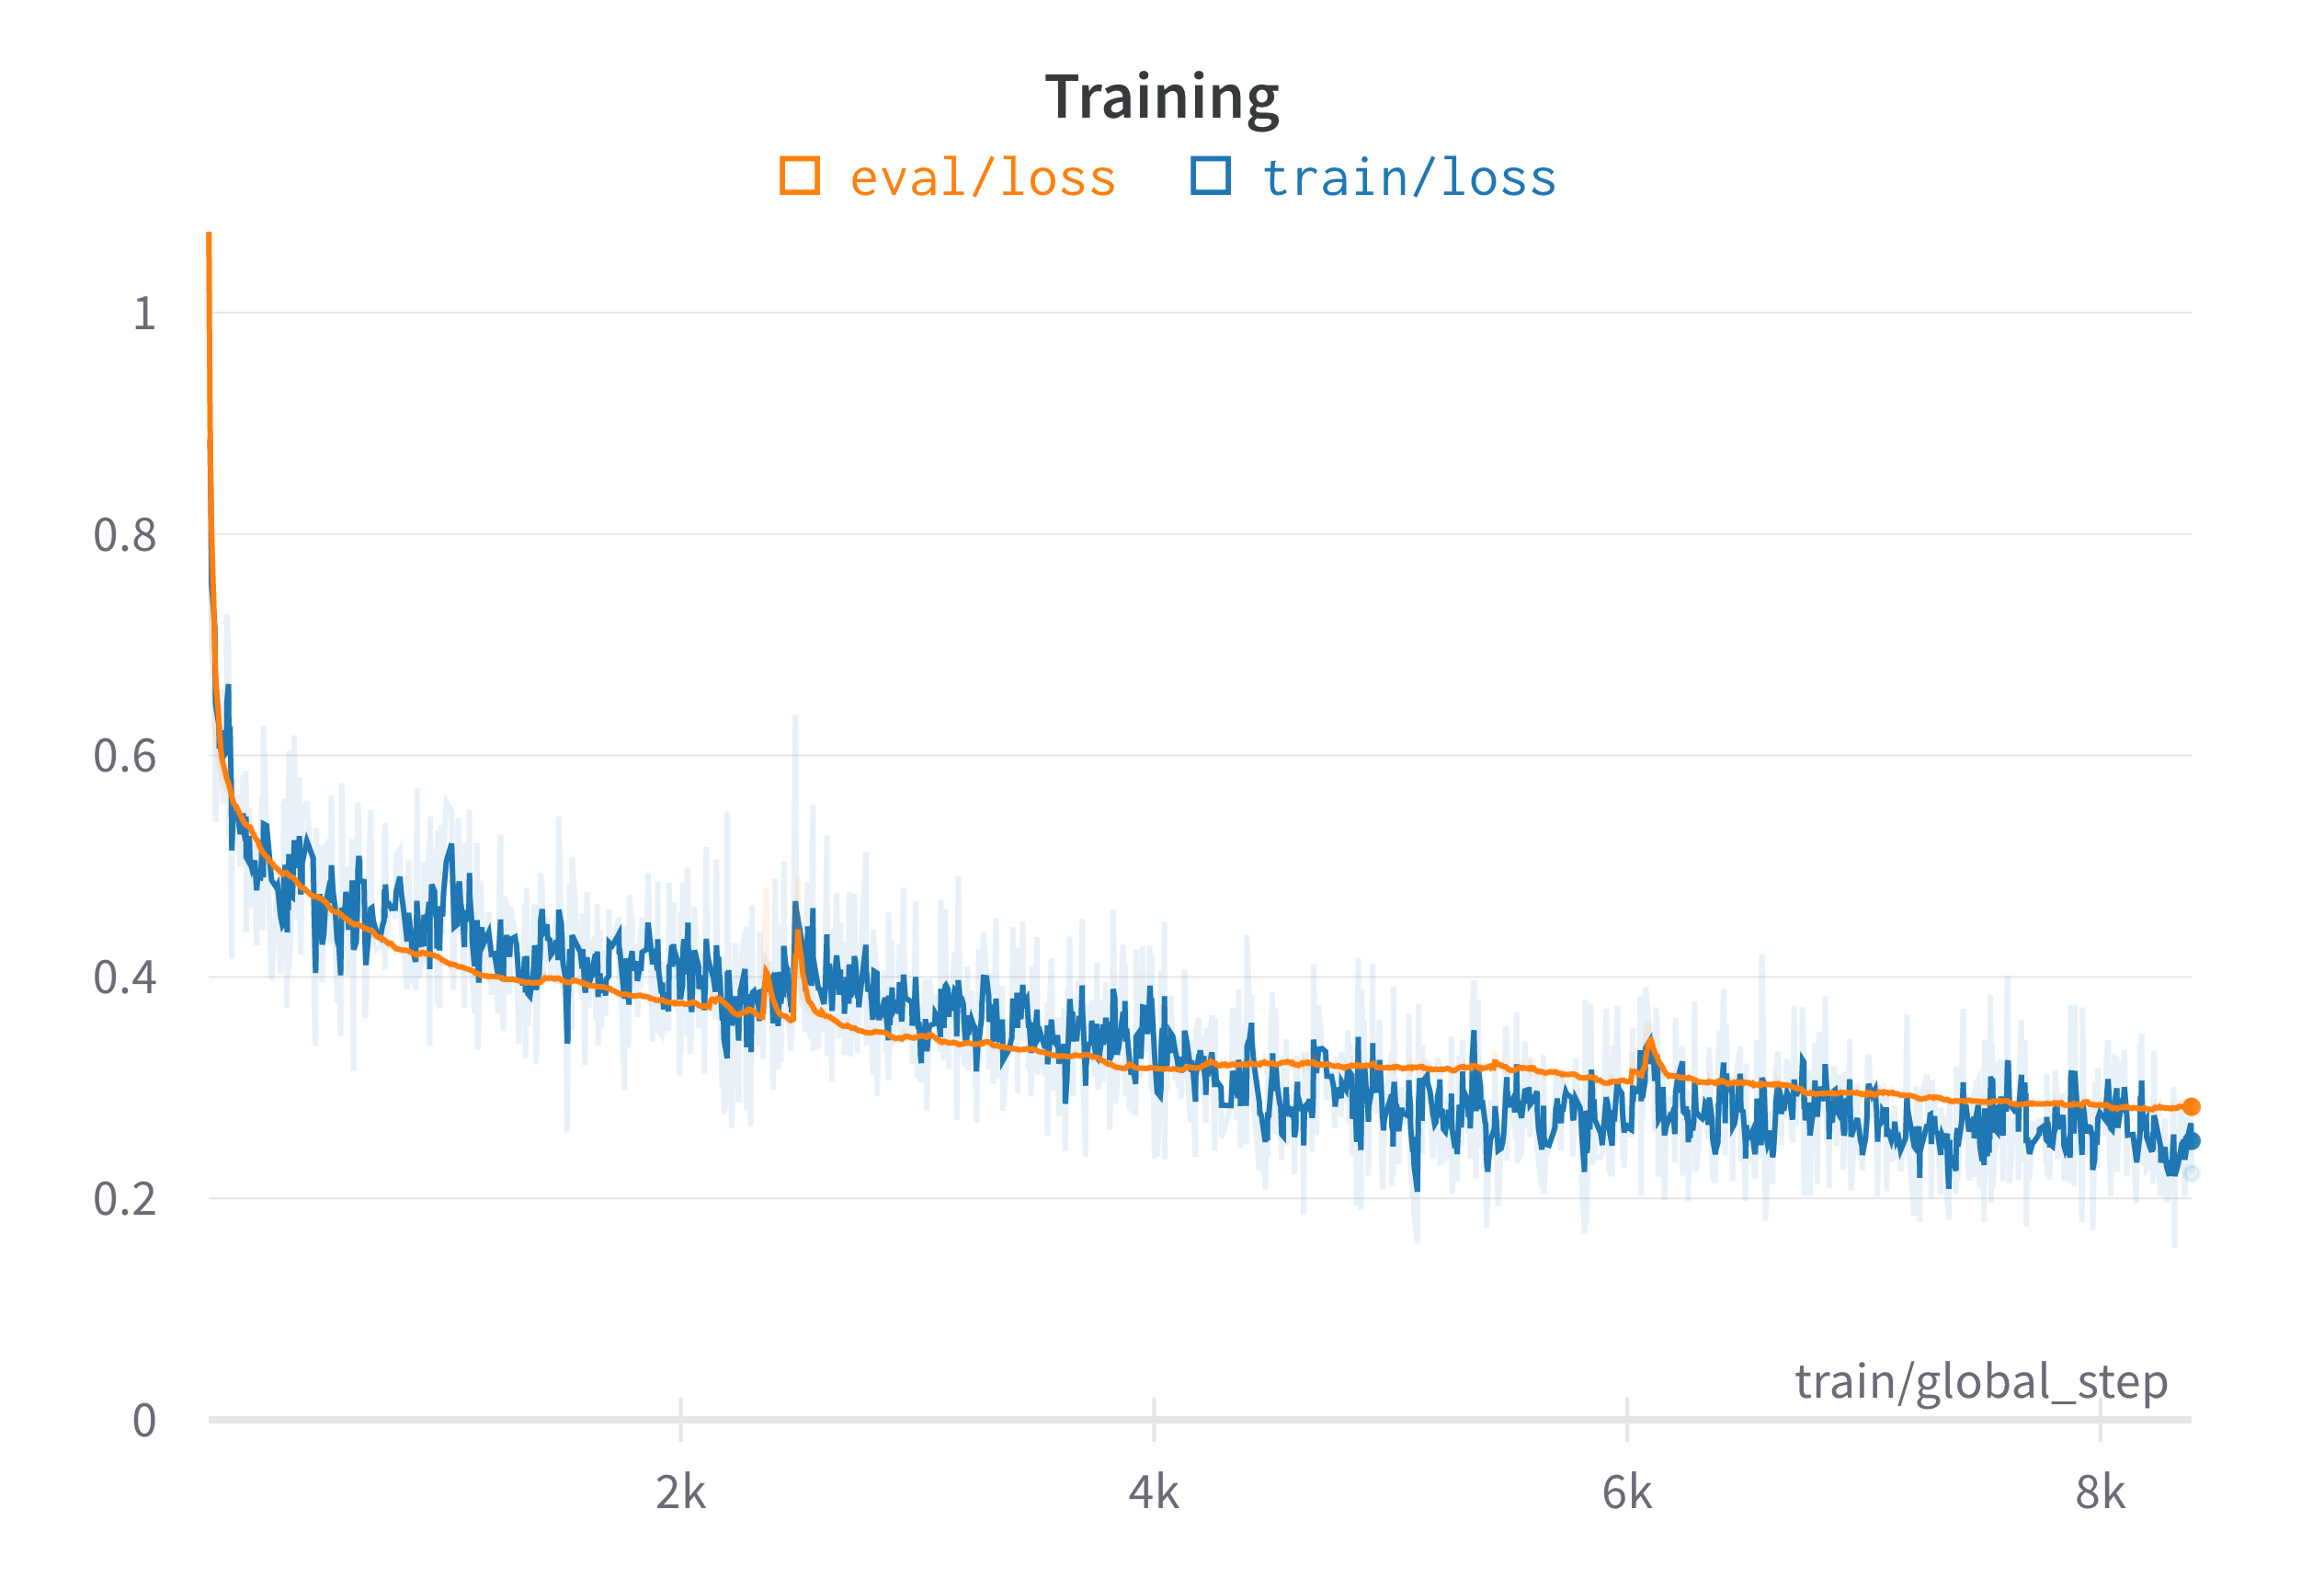
\includegraphics[width=\textwidth]{figures/wandb-train-loss-gpt-j-smart-contract.png}
    \caption{svg image}
\end{figure}

\begin{figure}[htp]
    \centering
    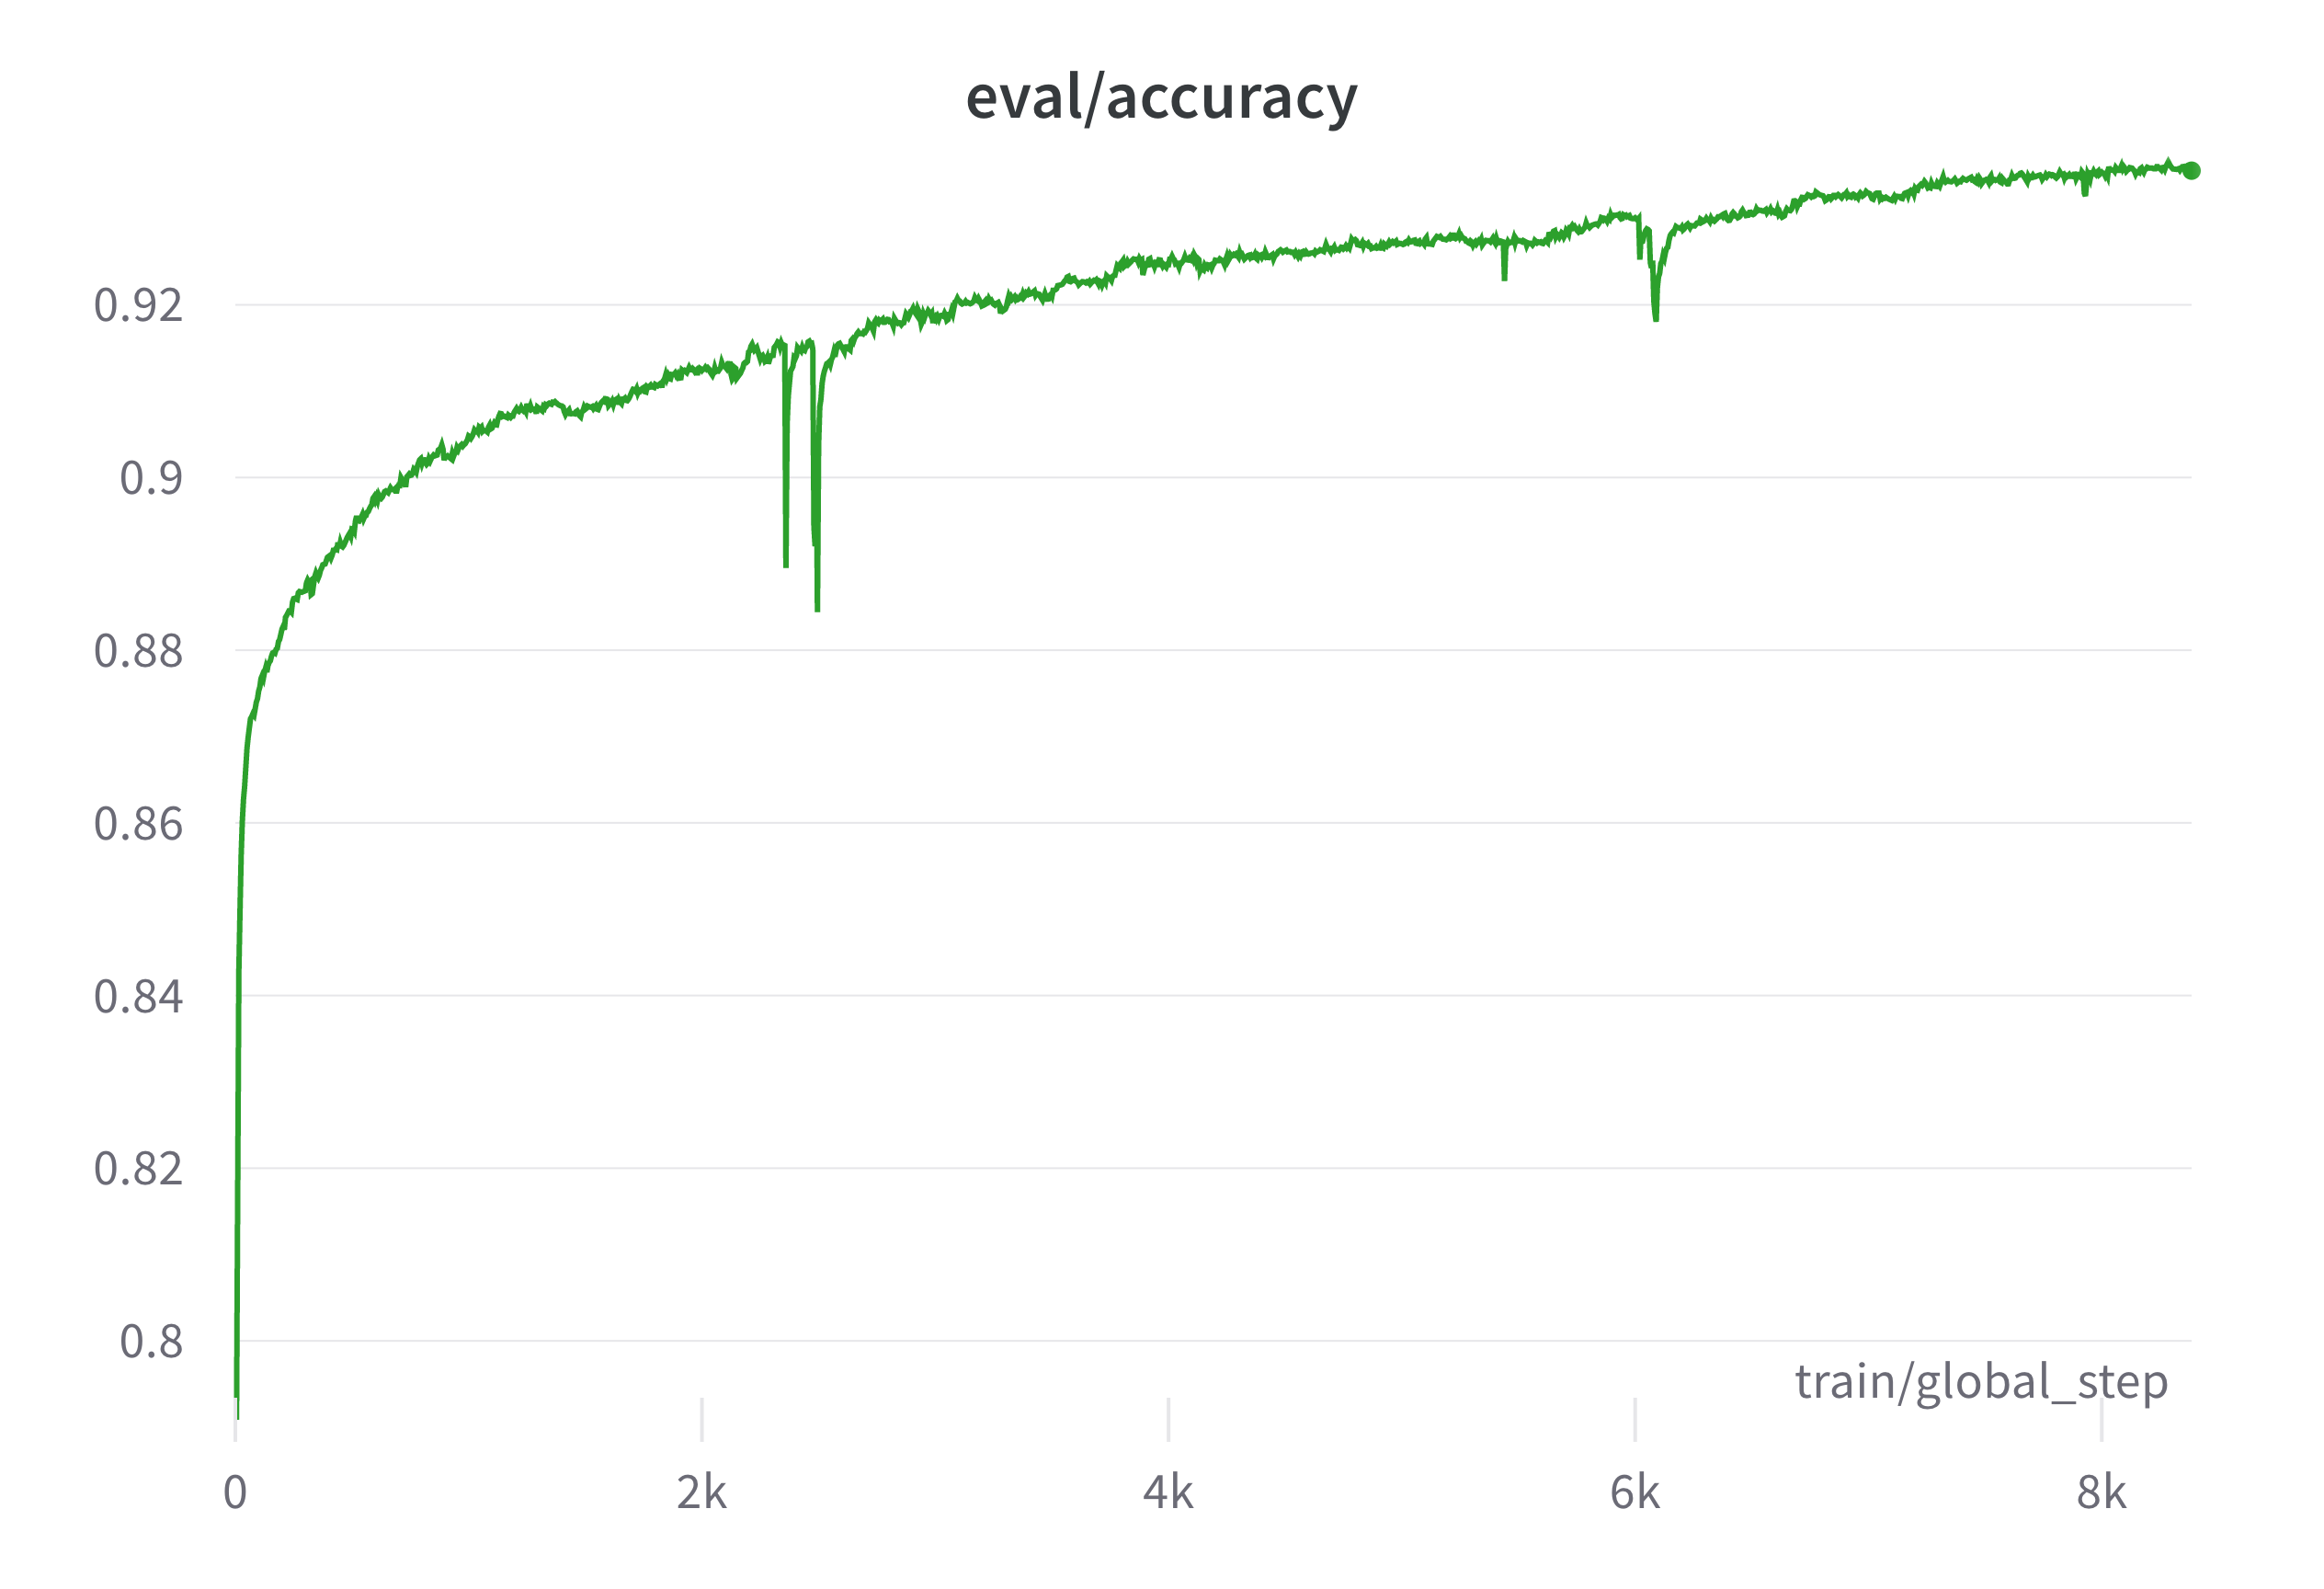
\includegraphics[width=\textwidth]{figures/wandb-train-eval-gpt-j-smart-contract.png}
    \caption{svg image}
\end{figure}

\section{Quantitative evaluation}

Even though only "HIH" severity vulnerabilities are labeled, several most of these also contain medium and low severity vulnerabilities. See Doughnut chart...  
The "full" context code is subject to latent vulnerabilities, which are unavoidable. Hence this could explain the low decrease in vulnerabilities.




\section{Qualitative evaluation}


\section{Memorisation evaluation}
Check if the model is just copying

Do this by investigating logits from  all layers.

Check common substrings in dattaset.

\section{Diff}

Tryto make custom generattion function that only selects SECURE solutions.....??

Does the temperature affect how secure solutions are?


Huugging face emojie as transformer model!


\section{Model weigts}

Can  we  find structures in the eriht? Neural  view? bertviz? That resembles AST equivalent?

